\let\lesson\undefined
\newcommand{\lesson}{\phantomlesson{Bài 16.}}
\setcounter{section}{2}
\section{Trắc nghiệm nhiều phương án lựa chọn}
\setcounter{ex}{0}
\Opensolutionfile{ans}[ans/VN10-Y24-PH-SYL-028P-TN]
% ===================================================================
\begin{ex}\mkstar{1}
	Hiệu suất là tỉ số giữa
	\choice
	{năng lượng hao phí và năng lượng có ích}
	{năng lượng có ích và năng lượng hao phí}
	{năng lượng hao phí và năng lượng toàn phần}
	{\True năng lượng có ích và năng lượng toàn phần}
	\loigiai{}
\end{ex}
% ===================================================================
\begin{ex}\mkstar{1}
Phát biểu nào sau đây là \textbf{không đúng} khi nói về hiệu suất?	
	\choice
	{Hiệu suất của động cơ luôn nhỏ hơn 1}
	{Hiệu suất đặc trưng cho mức độ hiệu quả của động cơ}
	{Hiệu suất của động cơ được xác định bằng tỉ số giữa công suất có ích và công suất toàn phần}
	{\True Hiệu suất được xác định bằng tỉ số giữa năng lượng đầu ra và năng lượng đầu vào}
	\loigiai{Hiệu suất được xác định bằng tỉ số giữa năng lượng đầu ra và năng lượng đầu vào.}
\end{ex}
% ===================================================================
\begin{ex}\mkstar{1}
Hiệu suất càng cao thì	
	\choice
	{tỉ lệ năng lượng hao phí so với năng lượng toàn phần càng lớn}
	{năng lượng tiêu thụ càng lớn}
	{năng lượng hao phí càng ít}
	{\True tỉ lệ năng lượng hao phí so với năng lượng toàn phần càng ít}
	\loigiai{}
\end{ex}
% ===================================================================
\begin{ex}\mkstar{2}
Hiệu suất của một quá trình chuyển hóa công được kí hiệu là $H$. Vậy $H$ luôn có giá trị	
	\choice
	{$H>1$}
	{$H=1$}
	{$H<1$}
	{\True $0<H\le 1$}
	\loigiai{}
\end{ex}
% ===================================================================
\begin{ex}\mkstar{2}
	Để nâng một tảng đá có trọng lượng $\SI{500}{\newton}$ lên như hình, một người sử dụng đòn bẩy bằng cách tác dụng một lực $\SI{180}{\newton}$ vào một đầu đòn bẩy làm cho đầu đòn bẩy dịch chuyển $\SI{70}{\centi\meter}$ còn tảng đá dịch chuyển $\SI{20}{\centi\meter}$. Hiệu suất của đòn bẩy là
	\begin{center}
		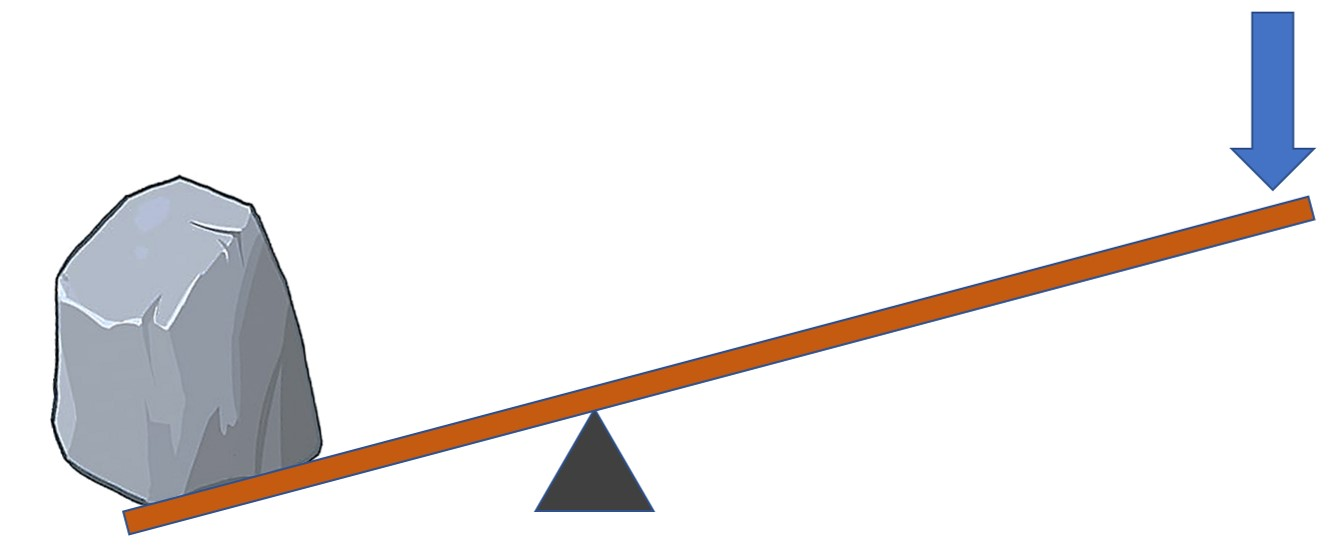
\includegraphics[width=0.4\linewidth]{../figs/VN10-2022-PH-TP023-P-12}
	\end{center}
	\choice
	{$\SI{126}{\percent}$}
	{$\SI{97.2}{\percent}$}
	{$\SI{36.0}{\percent}$}
	{\True $\SI{79.4}{\percent}$}
	\loigiai{}
\end{ex}
% ===================================================================
\begin{ex}\mkstar{2}
	Một động cơ có công suất tiêu thụ bằng $\SI{5}{\kilo\watt}$ kéo một vật có trọng lượng $\SI{12}{\kilo\newton}$ lên cao $\SI{30}{\meter}$ theo phương thẳng đứng trong thời gian $\SI{90}{\second}$ với vận tốc không đổi. Hiệu suất của động cơ bằng
	\choice
	{$\SI{100}{\percent}$}
	{\True $\SI{80}{\percent}$}
	{$\SI{60}{\percent}$}
	{$\SI{40}{\percent}$}
	\loigiai{Công cần thiết để kéo vật nặng lên cao $\SI{30}{\meter}$:
		$$A_i=Ph=\SI{360}{\kilo\joule}$$
		Công suất có ích để kéo vật:
		$$\calP_i=\dfrac{A_i}{t}=\SI{40}{\kilo\watt}$$
		Hiệu suất động cơ:
		$$H=\dfrac{\calP_i}{\calP_{tp}}\cdot\SI{100}{\percent}=\SI{80}{\percent}.$$}
\end{ex}
% ===================================================================
\begin{ex}\mkstar{3}
Một máy bơm nước mỗi giây có thể bơm được 15 lít nước lên bể ở độ cao $\SI{10}{\meter}$. Hiệu suất của máy bơm là 0,7. Lấy $g=\SI{10}{\meter/\second^2}$. Biết khối lượng riêng của nước là  $D=\SI{E3}{\kilogram/\meter^3}$. Sau nửa giờ máy bơm đã thực hiện một công bằng	
	\choice
	{$\SI{1500}{\kilo\joule}$}
	{\True $\SI{3857}{\kilo\joule}$}
	{$\SI{1890}{\kilo\joule}$}
	{$\SI{7714}{\kilo\joule}$}
	\loigiai{Khối lượng nước được bơm lên sau nửa giờ:
		$$m=D\cdot V=\left(\SI{1000}{\kilogram/\meter^3}\right)\cdot\left(\SI{15E-3}{\meter^3}\right)\cdot\left(\SI{1800}{\second}\right)=\SI{27E3}{\kilogram}$$
		Công có ích máy bơm cần thực hiện để bơm lượng nước trên lên cao $\SI{10}{\meter}$:
		$$A_i=mgh=\SI{2700}{\kilo\joule}$$
		Công toàn phần máy bơm thực hiện:
		$$A_\text{tp}=\dfrac{A_i}{H}=\SI{3857}{\kilo\joule}.$$}
\end{ex}
\Closesolutionfile{ans}
\section{Trắc nghiệm đúng/sai}
\setcounter{ex}{0}
\Opensolutionfile{ans}[ans/VN10-Y24-PH-SYL-028P-TF]
% ===================================================================
\begin{ex}
	Pin Mặt Trời hay pin quang điện được cấu tạo từ nhiều tế bào quang điện (solar cells). Các tế bào quang điện được chế tạo từ một loại chất liệu gọi là chất bán dẫn, thường thì chúng chế tạo từ silicon. Khi ánh sáng đi tới một tế bào quang điện, phần nhiều năng lượng của chúng bị tiêu hao. Một phần ánh sáng bị phản xạ hoặc truyền xuyên qua tế bào. Một phần bị chuyển thành nhiệt năng. Chỉ phần ánh sáng có màu sắc thích hợp là bị hấp thụ và sau đó chuyển hóa thành điện năng.
	\begin{center}
		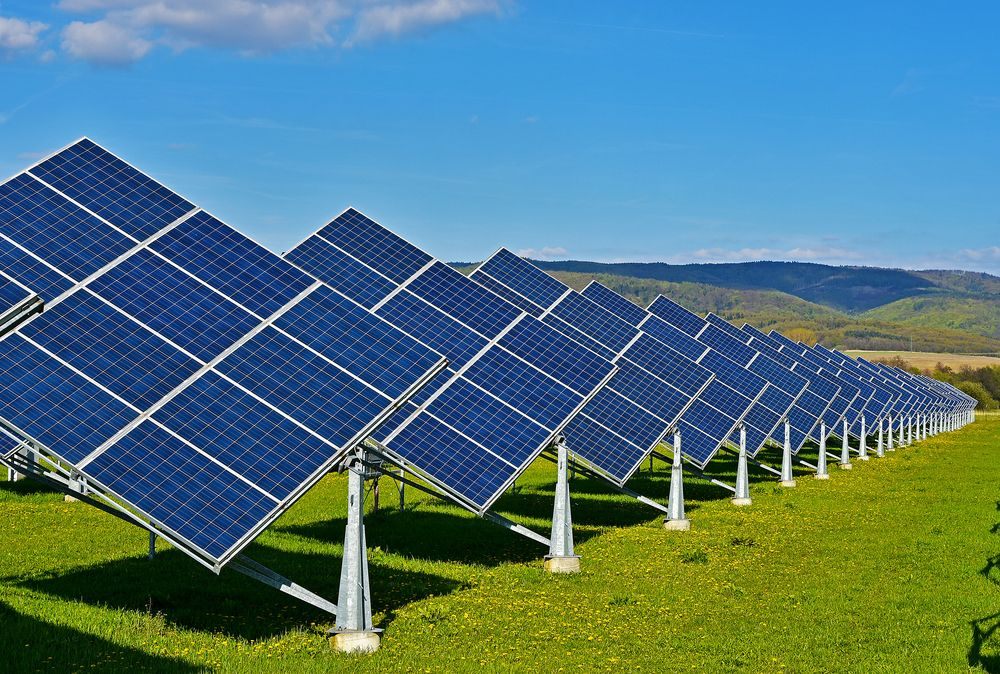
\includegraphics[width=0.4\linewidth]{../figs/VN10-2023-PH-TP028-1}
	\end{center}
	\choiceTF[t]
	{\True Pin Mặt Trời biến đổi quang năng thành điện năng}
	{Hiệu suất của pin mặt trời là tỷ số giữa quang năng mặt trời và nhiệt năng tỏa ra trên tấm pin}
	{\True Công suất bức xạ của Mặt Trời là $\SI{3.9E26}{\watt}$ thì  năng lượng Mặt Trời tỏa ra trong một ngày là $\SI{3.37E31}{\joule}$}
	{\True Hiệu suất pin mặt trời là $\SI{15}{\percent}$ thì để tạo ra $\SI{15}{\kilo\watt\hour}$ điện thì cần một lượng năng lượng mặt trời là $\SI{8.1}{\mega\joule}$
	}
	\loigiai{}
\end{ex}
% ===================================================================
\begin{ex}
	Người ta kéo một xô vật liệu $\SI{20}{\kilogram}$ lên tầng nhà đang thi công cách mặt đất $\SI{4}{\meter}$. Lực kéo có độ lớn không đổi $\SI{320}{\newton}$. Bỏ qua mọi ma sát. lấy $g=\SI{10}{\meter/\second^2}$, mốc thế năng tại mặt đất.
	\begin{center}
		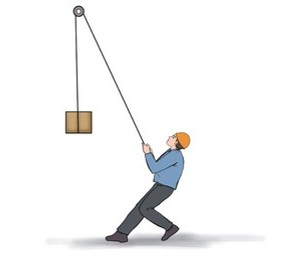
\includegraphics[width=0.4\linewidth]{../figs/VN10-2022-PH-TP028-2}
	\end{center}
	\choiceTF[t]
	{Vật liệu được kéo đều lên cao}
	{\True Thế năng của vật liệu khi đến độ cao $\SI{4}{\meter}$ là $\SI{800}{\joule}$}
	{\True Cơ năng của vật khi đến độ cao $\SI{4}{\meter}$ là $\SI{1.28}{\kilo\joule}$}
	{Hiệu suất của quá trình kéo vật là $\SI{37.5}{\percent}$}
	\loigiai{
	\begin{itemchoice}
		\itemch Sai. Vật liệu được kéo lên nhanh dần đều với gia tốc $a=\dfrac{F-mg}{m}=\SI{6}{\meter/\second^2}$.
		\itemch Đúng.
		\itemch Đúng.
		\itemch Sai. Hiệu suất của quá trình kéo $H=\dfrac{mg}{F}=\SI{62.5}{\percent}$.
	\end{itemchoice}
	}
\end{ex}
\Closesolutionfile{ans}
\section{Tự luận}
\setcounter{ex}{0}
\Opensolutionfile{ans}[ans/VN10-Y24-PH-SYL-028P-TL]
% ======================================================================
\begin{ex}\mkstar{2}
Máy tời điện đang hoạt động với công suất $\SI{1000}{W}$ đưa $\SI{100}{kg}$ vật liệu lên đều tới độ cao $\SI{16}{m}$ trong $\SI{20}{s}$. Tính hiệu suất của máy tời.	
	\loigiai{Năng lượng có ích:
	$$W_\text{ci} = mgh = \SI{16000}{J}.$$
		Năng lượng toàn phần của máy
		$$W = A = Pt = \SI{20000}{J}.$$
		Hiệu suất của máy tời là:
		$$H =\dfrac{W_\text{ci}}{W} =\SI{80}{\percent}.$$}
\end{ex}
% ======================================================================
\begin{ex}\mkstar{2}
Khi đưa một vật lên cao $\SI{2,5}{m}$ bằng mặt phẳng nghiêng, người ta phải thực hiện một công là $\SI{3600}{J}$. Biết hiệu suất của mặt phẳng nghiêng là $\SI{75}{\percent}$. Tính khối lượng của vật đó. Lấy $g = \SI{10}{m/s}^2$.	
	\loigiai{Ta có:
		$$H = \dfrac{W_\text{ci}}{W} = \dfrac{Ph}{A}.$$
		Trọng lượng của vật
		$$P = \dfrac{HA}{h} = \SI{1080}{N}.$$
Khối lượng của vật đó
	$$m = \dfrac{P}{g} = \SI{10,8}{kg}.$$}
\end{ex}
% ======================================================================
\begin{ex}\mkstar{2}
Một xe bán tải có khối lượng 1,5 tấn, hiệu suất chuyển hóa năng lượng của động cơ xe là $\SI{18}{\percent}$. Tìm số lít xăng cần dùng để tăng tốc từ trạng thái nghỉ đến tốc độ $\SI{15}{m/s}$. Biết năng lượng chứa trong 3,8 lít xăng là $\text{1,3}\cdot10^8\ \text{J}$.	
	\loigiai{Công động cơ cần thực hiện để xe tăng tốc lên $\SI{15}{\meter/\second}$ từ trạng thái nghỉ:
		$$A_{\text{i}}=\dfrac{1}{2}m\left(v^2-v^2_0\right)=\SI{168750}{\joule}.$$
		Hiệu suất là $18\%$ nên công thực tế mà xe bán tải phải bỏ ra là:
		$$A= \dfrac{A'}{\SI{18}{\percent}}= \SI{937500}{J}.$$
		Số lít xăng cần dùng là:
		$$937500 \cdot \dfrac{\text{3,8}}{\text{1,3}\cdot 10^8} = \text{0,027}\ \text{lít}.$$}
\end{ex}
% ======================================================================
\begin{ex}\mkstar{2}
	Công suất sử dụng điện trung bình của một gia đình là $\SI{0.5}{\kilo\watt}$. Biết năng lượng mặt trời khi chiếu trực tiếp đến bề mặt của pin mặt trời đặt nằm ngang có công suất trung bình là $\SI{100}{\watt}$ trên một mét vuông. Giả sử chỉ có $\SI{15}{\percent}$ năng lượng mặt trời được chuyển thành năng lượng có ích (điện năng). Hỏi cần một diện tích bề mặt pin mặt trời là bao nhiêu để có thể cung cấp đủ công suất điện cho gia đình này?
	\loigiai{
	o	$\SI{33.3}{\meter^2}$.
	}
\end{ex}
% ======================================================================
\begin{ex}\mkstar{3}
	Một ô tô chuyển động đều với vận tốc $\SI{54}{km/h}$ có thể đi được đoạn đường dài bao nhiêu khi tiêu thụ hết 60 lít xăng? Biết động cơ của ô tô có công suất $\SI{45}{kW}$; hiệu suất $25\%$; $\SI{1}{kg}$ xăng đốt cháy hoàn toàn tỏa ra nhiệt lượng bằng $\xsi{46\cdot 10^6}{J/kg}$ và khối lượng riêng của xăng là $\SI{700}{kg/m^3}$.
	\loigiai{Đổi $\SI{54}{km/h} = \SI{15}{m/s}; \SI{45}{kW} = \SI{45000}{W}.$\\		
		Gọi $s$ là quãng đường đi được khi động cơ tiêu thụ hết 60 lít xăng.\\		
		Khối lượng 60 lít xăng:
		$$m = DV = \SI{42}{kg}.$$
		Công thực hiện của động cơ:
		$$A = \calP t = \calP \dfrac{s}{v}.$$
		Nhiệt lượng do 60 lít xăng khi bị đốt cháy hoàn toàn tỏa ra là 
		$$Q = qm.$$
		Ta có:
		$$H = \dfrac{A}{Q} \Rightarrow A = HQ  \Leftrightarrow P \dfrac{s}{v} = Hqm \Rightarrow s = \SI{161000}{m} = \SI{161}{km}.$$
		Vậy khi tiêu thụ hết 60 lít xăng, ô tô có thể đi được quãng đường là $\SI{161}{km}.$}
\end{ex}
% ======================================================================
\begin{ex}\mkstar{3}
	Một ô tô có khối lượng $m=\SI{1.25}{\text{tấn}}$ chuyển động nhanh dần đều từ trạng thái nghỉ cho đến khi đạt tốc độ $v=\SI{54.0}{\kilo\meter/\hour}$ thì chuyển động thẳng đều. Biết rằng trong quá trình tăng tốc ô tô đi được quãng đường có độ dài $s=\SI{800}{\meter}$.
	\begin{enumerate}[label=\alph*)]
		\item Tính động năng của ô tô trong giai đoạn nó chuyển động thẳng đều.
		\item Tính động năng của ô tô ngay khi nó đã tăng tốc được một khoảng thời gian $\tau=\SI{10}{\second}$.
		\item Tính động năng của ô tô ngay khi nó đã đi được quãng đường $s'=\SI{200}{\meter}$ tính từ lúc bắt đầu xuất phát.
		\item Tính công suất của động cơ ô tô khi nó có vận tốc $v'=\SI{10.0}{\meter/\second}$ biết rằng hiệu suất của động cơ ở vận tốc này là $\eta=\SI{70}{\percent}$.
	\end{enumerate}
	\loigiai{
	\begin{enumerate}[label=\alph*)]
		\item Động năng ô tô trong giai đoạn chuyển động thẳng đều $W=\dfrac{1}{2}mv^2\approx\SI{141}{\kilo\joule}.$
		\item Gia tốc của ô tô: $a=\dfrac{v^2}{2s}$\\
		Vận tốc của ô tô sau khoảng thời gian $\tau$:
		$$v_{\tau}=a\tau=\dfrac{v^2\tau}{2s}.$$
		Động năng của ô tô sau khoảng thời gian $\tau$
		$$W_{\text{đ}}=\dfrac{1}{2}mv^2_{\tau}=\dfrac{1}{8}\dfrac{mv^4\tau^2}{s^2}\approx\SI{1.24}{\kilo\joule}.$$
		\item Vận tốc của ô tô khi nó đi được quãng đường $s$
		$$v_{s'}=\sqrt{2as'}=v\sqrt{\dfrac{s'}{s}}\Rightarrow W'_{\text{đ}}=\dfrac{1}{2}mv^2_{s'}=\dfrac{1}{2}\dfrac{s'}{s}mv^2\approx\SI{35.2}{\kilo\joule}.$$
		\item Công suất có ích mà ô tô nhận được khi nó có vận tốc $v'=\SI{10.0}{\meter/\second}$
		$$\calP_i=Fv'=mav'=\dfrac{mv^2v'}{2s}=\eta \calP_{\text{đc}}.$$
		Công suất của động cơ ô tô khi đó:
		$$\calP_{\text{đc}}=\dfrac{\calP_i}{\eta}=\dfrac{mv^2v'}{2s\eta}\approx\SI{2.51}{\kilo\watt}.$$
	\end{enumerate}
	}
\end{ex}
% ======================================================================
\begin{ex}\mkstar{3}
	Động cơ xăng của ô tô có hiệu suất $\SI{27}{\percent}$. Điều này có nghĩa là chỉ $\SI{27}{\percent}$ năng lượng được lưu trữ trong nhiên liệu của ô tô được sử dụng để ô tô chuyển động (sinh công thắng lực ma sát).
	\begin{enumerate}[label=\alph*)]
		\item Biết một lít xăng dự trữ năng lượng $\SI{30}{\mega\joule}$. Năng lượng trong 1 lít xăng mà ô tô sử dụng được để chuyển động là bao nhiêu $\si{\mega\joule}$?
		\item Một ô tô dùng 1 lít xăng đi được $
		\SI{7}{\kilo\meter}$ với vận tốc không đổi $\SI{10}{\meter/\second}$. Tính độ lớn lực ma sát tác dụng lên ô tô.
	\end{enumerate}
	\loigiai{
	\begin{enumerate}[label=\alph*)]
		\item $A_i=\SI{27}{\percent}\cdot W=\SI{27}{\percent}\cdot 30=\SI{8.1}{\mega\joule}$.
		\item Độ lớn lực ma sát tác dụng lên ô tô:
		$$F_{\text{ms}}s=\SI{8.1}{\mega\joule}\Rightarrow F_{\text{ms}}=\SI{1.16}{\kilo\newton}.$$
	\end{enumerate}
	}
\end{ex}
\Closesolutionfile{ans}